%% LyX 2.3.4.2 created this file.  For more info, see http://www.lyx.org/.
%% Do not edit unless you really know what you are doing.
\documentclass[11pt,english]{article}
\usepackage{mathpazo}
\renewcommand{\ttdefault}{txtt}
\usepackage[latin9]{inputenc}
\usepackage{geometry}
\geometry{verbose,tmargin=2cm,bmargin=2cm,lmargin=2cm,rmargin=2cm}
\setlength{\parskip}{\smallskipamount}
\setlength{\parindent}{0pt}
\synctex=-1
\usepackage{babel}
\usepackage{array}
\usepackage{float}
\usepackage{booktabs}
\usepackage{units}
\usepackage{textcomp}
\usepackage{mathtools}
\usepackage{multirow}
\usepackage{amsmath}
\usepackage{graphicx}
\usepackage{setspace}
\usepackage[authoryear]{natbib}
\setstretch{1.05}
\usepackage[unicode=true,
 bookmarks=true,bookmarksnumbered=false,bookmarksopen=false,
 breaklinks=false,pdfborder={0 0 0},pdfborderstyle={},backref=false,colorlinks=false]
 {hyperref}
\hypersetup{pdftitle={Geofluids Project - Calculating the solubility of CO2 and calcite in brine using a Gibbs energy minimization approach},
 pdfauthor={Allan Leal}}

\makeatletter

%%%%%%%%%%%%%%%%%%%%%%%%%%%%%% LyX specific LaTeX commands.
\newcommand{\noun}[1]{\textsc{#1}}
%% Because html converters don't know tabularnewline
\providecommand{\tabularnewline}{\\}
\floatstyle{ruled}
\newfloat{algorithm}{tbp}{loa}
\providecommand{\algorithmname}{Algorithm}
\floatname{algorithm}{\protect\algorithmname}

%%%%%%%%%%%%%%%%%%%%%%%%%%%%%% User specified LaTeX commands.
%===================================================================
% General packages
%===================================================================
\usepackage[labelfont=bf]{caption}
\usepackage{tcolorbox}

%===================================================================
% Code listing and highlighting
%===================================================================
%\usepackage{listing}
%\usepackage{minted}
%\usemintedstyle{trac}
%
%\definecolor{light-gray}{gray}{0.98}
%
%%\newminted{python}{fontsize=\normalsize, linenos, numbersep=4pt, frame=lines, framesep=1mm} 
%\newminted{python}{bgcolor=light-gray, frame=none, framesep=1em} 
%
%\newminted{yaml}{fontsize=\scriptsize, 
%   linenos,
%   numbersep=4pt,
%   frame=lines,
%   framesep=1mm} 

%===================================================================
% Listings
%===================================================================

\usepackage{listings}
\usepackage{xcolor}

\definecolor{codegreen}{rgb}{0,0.6,0}
\definecolor{codegray}{rgb}{0.5,0.5,0.5}
\definecolor{codepurple}{rgb}{0.58,0,0.82}
\definecolor{backcolour}{rgb}{0.95,0.95,0.92}

\lstdefinestyle{mystyle}{
	backgroundcolor=\color{backcolour},   
	commentstyle=\color{codegreen},
	keywordstyle=\color{magenta},
	numberstyle=\tiny\color{codegray},
	stringstyle=\color{codepurple},
	basicstyle=\ttfamily\footnotesize,
	breakatwhitespace=false,         
	breaklines=true,                 
	captionpos=b,                    
	keepspaces=true,                 
	numbers=left,                    
	numbersep=5pt,                  
	showspaces=false,                
	showstringspaces=false,
	showtabs=false,                  
	tabsize=2
}

\lstset{style=mystyle}

%===================================================================
% Algorithm listing
%===================================================================
\usepackage{algorithm}
\usepackage{algorithmicx}
\usepackage[noend]{algpseudocode} % without `end for`, `end if`, etc.

\makeatother

\begin{document}
\title{\rule[0.5ex]{1\columnwidth}{2pt}{\Huge{}}\\
\noun{\Huge{}geofluids project}\\
Calculating the solubility of CO$_{2}$ and calcite in brine using
a Gibbs energy minimization approach\\
\rule[0.5ex]{1\columnwidth}{2pt}}
\author{Lecturer: Dr. Allan Leal}
\maketitle

\section{Introduction}

\begin{table}
\begin{centering}
\caption{\label{tab:chemical-system-example}The chemical system considered
in the given Python code to calculate solubility of CO$_{2}$ and
CaCO$_{3}$ in NaCl brine.}
\par\end{centering}
\centering{}%
\begin{tabular*}{1\columnwidth}{@{\extracolsep{\fill}}ccccccccc}
\toprule 
\multicolumn{2}{c}{Species} &  & \multicolumn{2}{c}{Phases} &  & \multicolumn{3}{c}{Components}\tabularnewline
\midrule
$\alpha_{1}$ & H$_{2}$O(l) &  & \multirow{9}{*}{$\pi{}_{1}$} & \multirow{9}{*}{Aqueous} &  & $\varepsilon{}_{1}$ & H & \emph{hydrogen}\tabularnewline
$\alpha_{2}$ & H$^{+}$(aq) &  &  &  &  & $\varepsilon{}_{2}$ & O & \emph{oxygen}\tabularnewline
$\alpha_{3}$ & OH$^{-}$(aq) &  &  &  &  & $\varepsilon{}_{3}$ & C & \emph{carbon}\tabularnewline
$\alpha_{4}$ & HCO$_{3}^{-}$(aq) &  &  &  &  & $\varepsilon{}_{4}$ & Na & \emph{sodium}\tabularnewline
$\alpha_{5}$ & CO$_{3}^{2-}$(aq) &  &  &  &  & $\varepsilon{}_{5}$ & Cl & \emph{chlorine}\tabularnewline
$\alpha_{6}$ & CO$_{2}$(aq) &  &  &  &  & $\varepsilon{}_{6}$ & Ca & \emph{calcium}\tabularnewline
$\alpha_{7}$ & Na$^{+}$(aq) &  &  &  &  & $\varepsilon{}_{7}$ & Z & \emph{electric charge}\tabularnewline
$\alpha_{8}$ & Cl$^{-}$(aq) &  &  &  &  &  &  & \tabularnewline
$\alpha_{9}$ & Ca$^{2+}$(aq) &  &  &  &  &  &  & \tabularnewline
$\alpha_{10}$ & CO$_{2}$(g) &  & \multirow{1}{*}{$\pi{}_{2}$} & \multirow{1}{*}{Gaseous} &  &  &  & \tabularnewline
$\alpha_{11}$ & CaCO$_{3}$(s, calcite) &  & $\pi{}_{3}$ & Calcite &  &  &  & \tabularnewline
\bottomrule
\end{tabular*}
\end{table}

In this project, a Python code for chemical equilibrium calculations
for the chemical system shown in Table~\ref{tab:chemical-system-example},
based on a Gibbs energy minimization approach, is given. This code
needs to be improved and then used for solubility calculations of
carbon dioxide (CO$_{2}$) and calcite (CaCO$_{3}$) in saline water.
The improvement includes:
\begin{enumerate}
\item The implementation of more accurate models for the activities, $a_{i}$,
of aqueous and gaseous species to replace the current ones based on
ideal solution and idea gas models. The activity models to be implemented
in this project were explained in class, and they are also detailed
in Section~\ref{sec:implementing-activity-models}. These activity
models are essential for more accurate chemical equilibrium calculations
because they are either based on more realistic theoretical models
governing the chemistry of fluids or because they are models calibrated
with experimental data.
\item The implementation of an interpolation scheme for the calculation
of standard chemical potentials of the species, $\mu_{i}^{\circ}$,
at temperatures and pressures other than only 25~°C and 1~bar. This
interpolation capability will extend the temperature and pressure
range capability of the code; permit more accurate equilibrium calculations,
and thus solubility calculations, at higher temperatures and pressures;
and allow one to identify how increasing temperature and pressure
affect the solubility of CO$_{2}$ and CaCO$_{3}$.
\end{enumerate}
Once the required model improvements have been carried out in the
code, use it to perform chemical equilibrium calculations whose resulting
equilibrium state (i.e., the molar amounts, activities, and concentrations
of the species at equilibrium) can be appropriately used to plot the
missing curves in the figure templates shown in Figure~\ref{fig:assigned-figures}.
This should require some additional code to automate the process of
\emph{(i)} performing the equilibrium calculation, \emph{(ii)} extracting
the appropriate data from the calculated equilibrium state, \emph{(iii)}
and define plots using Python\emph{.} 

These coding and modeling tasks can be accomplished in groups of two
students (exceptionally three students maximum). A written report
is required, in which the produced figures, using the templates shown
in Figure~\ref{fig:assigned-figures}, are presented along with a
brief explanation of each of them (e.g., an increase in X results
from an increase in Y because of ..., or, which implies in higher/lower
..., etc.). The report should also have a brief personal statement
of each group member explaining his/her contribution. Both the written
report, containing the names of the students, and the modified Python
code should be \textbf{submitted using Moodle by the last day of course}. 
\begin{center}
\textbf{The written report should also be printed, signed, and handed
to me by that day.}
\par\end{center}

\begin{figure}
\begin{centering}

\includegraphics{figures/figures-for-project}
\par\end{centering}
\caption{\label{fig:assigned-figures}The figures that need to be plot in this
project. }
\end{figure}


\section{Implementing activity models for aqueous and gaseous species\label{sec:implementing-activity-models}}

The provided code calculates the equilibrium state of the chemical
system in Table~\ref{tab:chemical-system-example} by solving the
following Gibbs energy minimization problem:
\begin{equation}
\min_{n}G=\sum_{i=1}^{\text{N}}n_{i}\mu_{i}\quad\text{subject to}\quad An=b\quad\text{and}\quad n\geq0.\label{eq:gibbs-mim-problem}
\end{equation}
This minimization problem can be converted into a \emph{system of
non-linear equations}, which can then be solved using \emph{Newton's
method}. The minimization problem consists in calculating the molar
amounts of the species, ${n=(n_{1},\ldots,n_{\mathrm{N}})}$, that
minimizes the Gibbs energy of the system, $G$. However, this minimization
calculation needs to be performed with two constraints. The first
constraint imposes that the amounts of the species, $n$, need to
satisfy the equation:
\begin{equation}
An=b,
\end{equation}
i.e., the amounts of the species at equilibrium must preserve the
given amounts of the elements, here denoted by ${b=(b_{1},\ldots,b_{\mathrm{E}})}$.
The second constraint imposes that the amounts of the species at equilibrium
is non-negative:
\begin{equation}
n\geq0,
\end{equation}
with the above inequality constraint meaning that ${n_{i}\geq0}$
for all species ${i=1,\ldots,\mathrm{N}}$. 

The \emph{chemical potential} of the species, $\mu_{i}$, is defined
as:
\begin{equation}
\mu_{i}=\mu_{i}^{\circ}+RT\ln a_{i},
\end{equation}
where $\mu_{i}^{\circ}$ is the \emph{standard chemical potential}
of the $i$th species; ${R=\unit[8.31446]{J/mol}}$ is the universal
gas constant; $T$ is temperature; and $a_{i}$ is the \emph{activity}
of the $i$th species. 

The standard chemical potentials of the species, $\mu_{i}^{\circ}$,
depend only on temperature, $T$, and pressure, $P$. Section~\ref{subsec:Implementing-interpolation-funct}
provides values for these thermodynamic properties at various temperatures
and pressures for all chemical species considered in this project
(see Table~\ref{tab:standard-chemical-potentials}). 

The activities of the species, $a_{i}$, can be thought as their effective
concentrations, i.e., their concentrations corrected for the non-ideal
behavior of solutions. They are calculated differently for each phase.
Section~\ref{subsec:activity-model-aqueous} describe activity models
for aqueous species, and Section~\ref{subsec:activity-model-gaseous}
for CO$_{2}$(g).

\subsection{Activity model for aqueous solution\label{subsec:activity-model-aqueous}}

\begin{figure}
\begin{centering}

\includegraphics[width=12cm]{figures/activity-coefficient-davies}
\par\end{centering}
\caption{\label{fig:activity-coefficient-ions}Activity coefficients of ionic
species, $\gamma_{i}$, using Davies model.}
\end{figure}

\begin{figure}
\begin{centering}
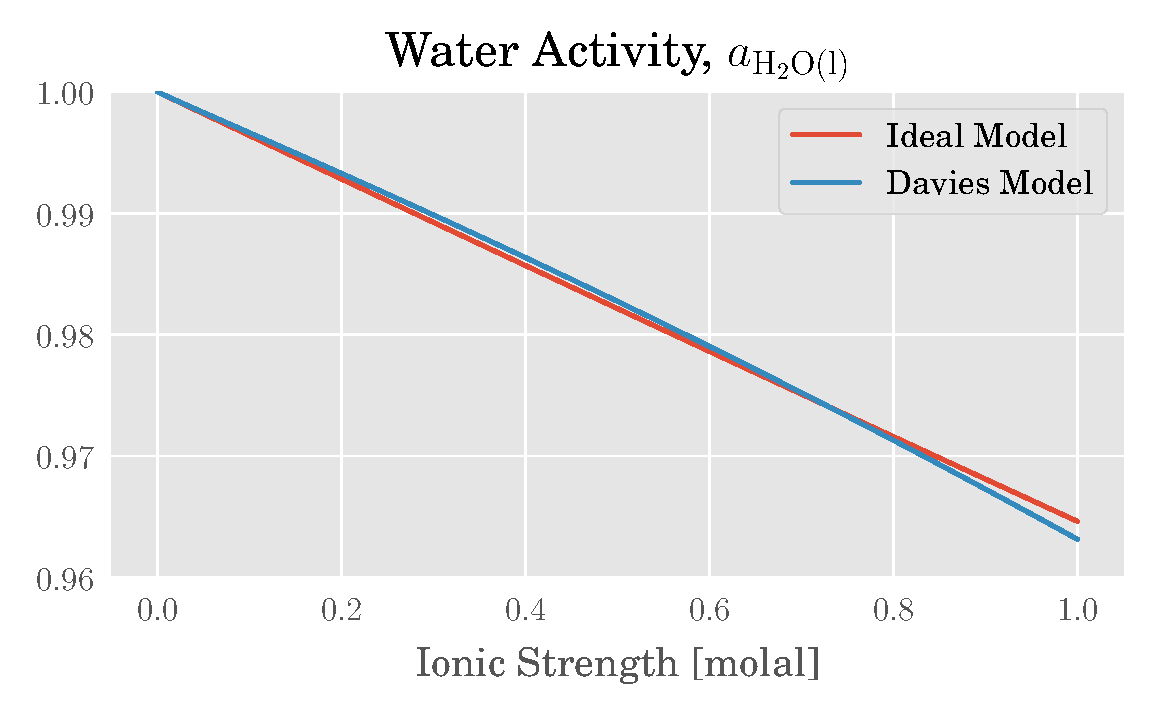
\includegraphics[width=12cm]{figures/activity-water-davies}
\par\end{centering}
\caption{\label{fig:activity-water-davies}Activity of water species, $a_{\mathrm{H_{2}O(l)}}$,
using both a Davies model and an ideal solution model.}
\end{figure}

\begin{figure}
\begin{centering}

\includegraphics[width=12cm]{figures/activity-coefficient-co2-drummond}
\par\end{centering}
\caption{\label{fig:activity-coefficient-co2-drummond}Activity coefficient
of dissolved CO$_{2}$ species, $\gamma_{\mathrm{CO_{2}(aq)}}$, using
\citet{drummond1981boiling} model.}
\end{figure}

In an aqueous solution, the species H$_{2}$O(l) is referred to as
the \emph{solvent species}, and all other species are \emph{solute
species}, e.g., Na$^{+}$(aq), HCO$_{3}^{-}$(aq), CO$_{2}$(aq).
The solute species can be \emph{ions}, electrically charged species,
such as H$^{+}$(aq) and CO$_{3}^{2-}$(aq), with charges $+1$ and
$-2$, respectively; or they can be \emph{neutral}, such as CO$_{2}$(aq).
In what follows, we describe \emph{activity models} for aqueous solute
species, for both ions and neutral solutes, as well as for aqueous
solvent species, H$_{2}$O(l). Before activity models for these species
are presented, however, some important definitions of concentration
measures for aqueous solutions are presented.

\subsubsection*{Molality of aqueous solute species}

The concentration measure most commonly used for aqueous solutes is
\emph{molality}. The molality of a solute is represented by $m_{i}$
and defined as:
\begin{equation}
m_{i}=\frac{n_{i}}{M_{\mathrm{H_{2}O(l)}}},
\end{equation}
where $M_{\mathrm{H_{2}O(l)}}$ is the mass of solvent water, the
species H$_{2}$O(l), in kg. The unit of molality is \emph{molal},
or equivalently mol/kgw, i.e., the number of moles of a solute divided
by the mass, in kg, of solvent water, the species H$_{2}$O(l). For
solvent water, the molality concentration is not defined, and certainly
not useful. Why?

Using the molar mass of water, ${\mathcal{M}_{\mathrm{H_{2}O}}=\unit[18.01528\cdot10^{-3}]{kg/mol}}$,
we can use instead the following equation to calculate the molality
of solutes:
\begin{equation}
m_{i}=55.5084\frac{n_{i}}{n_{\mathrm{H_{2}O(l)}}}.
\end{equation}


\subsubsection*{Ionic strength of the aqueous solution}

An aqueous solution can exist at infinitely many different compositions
(i.e., different concentrations for the solutes). However, when the
aqueous solution is sufficiently diluted, with low concentrations
of solutes, two diluted aqueous solutions with different composition
tend to behave similarly, thermodynamically, when its \emph{ionic
strength}, denoted by $I$, is the same. The ionic strength of an
aqueous solution is defined as:
\begin{equation}
I=\frac{1}{2}\sum_{i=1}^{\mathrm{N^{aq}}}m_{i}Z_{i}^{2},
\end{equation}
where $Z_{i}$ is the \emph{electrical charge} of the $i$th aqueous
species; and $\mathrm{N^{aq}}$ is the number of aqueous species. 

\subsubsection*{Activity of ionic aqueous solute species}

The activity of aqueous ionic species is defined as:
\begin{equation}
a_{i}=\gamma_{i}m_{i},
\end{equation}
where $\gamma_{i}$ is the \emph{activity coefficient} of the ionic
species. The activity coefficient can be seen as a factor that corrects
the species concentration for the non-ideal thermodynamic behavior
of aqueous solutions. In the provided Python code, ${\gamma_{i}=1}$,
which corresponds to an assumption that the saline water, i.e., brine,
is an ideal solution according to thermodynamics. 

In this project, the \emph{Davies activity model} needs to be used
to calculate $\gamma_{i}$ for aqueous ions as follows:
\begin{equation}
\log_{10}\gamma_{i}=-A_{\gamma}Z_{i}^{2}\left(\dfrac{\sqrt{I}}{1+\sqrt{I}}-0.3I\right),
\end{equation}
where $A_{\gamma}$ is a Debye\textendash Hückel parameter defined
as:
\begin{equation}
A_{\gamma}=1.824928\cdot10^{6}\rho_{\mathrm{H_{2}O}}^{1/2}(\epsilon_{\mathrm{H_{2}O}}T)^{-3/2},
\end{equation}
where $\rho_{\mathrm{H_{2}O}}$ and $\epsilon_{\mathrm{H_{2}O}}$
are the density and dielectric constant of pure water. In this project,
use ${A_{\gamma}=0.5095}$, which corresponds to its value at 25~°C
and 1~bar. See Figure~\ref{fig:activity-coefficient-ions}. 

\begin{tcolorbox}

\textbf{Note:} You'll need to convert from $\log_{10}$ to $\ln$
in the code. Use
\[
\ln\gamma_{i}=2.30258\log_{10}\gamma_{i},
\]
where 2.30258 is an approximation for $\ln10$. \end{tcolorbox}

\subsubsection*{Activity of aqueous solvent species H$_{2}$O(l)}

The activity of the aqueous species H$_{2}$O(l) can be calculated
using:
\begin{equation}
\ln a_{\mathrm{H_{2}O(l)}}=\frac{\ln10}{55.5084}A\left[2\left(\frac{I+2\sqrt{I}}{1+\sqrt{I}}\right)-4\ln(1+\sqrt{I})-0.3I^{2}\right]-\frac{1-x_{\mathrm{H_{2}O(l)}}}{x_{\mathrm{H_{2}O(l)}}},
\end{equation}
where $x_{\mathrm{H_{2}O(l)}}$ is the mole fraction of H$_{2}$O(l).
This equation results in activity values for solvent water that satisfies
the Gibbs\textendash Duhem equation when the Davies model is used
for the activities of ionic species (\emph{not addressed in this course}).
However, we saw in class that for the range of ionic strengths for
which the Davies model is valid, 0.1\textendash 0.7 molal, the above
equation and the following one for an ideal solution model results
in very similar values (see Figure~\ref{fig:activity-water-davies}):
\begin{equation}
\ln a_{\mathrm{H_{2}O(l)}}=-\frac{1-x_{\mathrm{H_{2}O(l)}}}{x_{\mathrm{H_{2}O(l)}}}.
\end{equation}


\subsubsection*{Activity of neutral aqueous solute species CO$_{2}$(aq)}

The activity of the aqueous species CO$_{2}$(aq) can be calculated
using:
\begin{equation}
a_{\mathrm{CO_{2}(aq)}}=\gamma_{\mathrm{CO_{2}(aq)}}m_{\mathrm{CO_{2}(aq)}},
\end{equation}
with the activity coefficient of CO$_{2}$(aq) calculated using \citet{drummond1981boiling}
model:
\begin{equation}
\ln\gamma_{\mathrm{CO_{2}}}=\left(c_{1}+c_{2}T+\frac{c_{3}}{T}\right)I-(c_{4}+c_{5}T)\frac{I}{I+1},
\end{equation}
where ${c_{1}=-1.0312}$, ${c_{2}=1.2806\cdot10^{-3}}$, ${c_{3}=255.9}$,
${c_{4}=0.4445}$ and ${c_{5}=-1.606\cdot10^{-3}}$; $T$ is temperature
in units of K; and $I$ is the ionic strength of the aqueous solution
in units of molal. This equation is valid within the temperature and
salinity ranges 20\textendash 400~°C and 0\textendash 6.5~molal
respectively. See Figure~\ref{fig:activity-coefficient-co2-drummond}.

\subsection{Activity model for gaseous solution\label{subsec:activity-model-gaseous}}

\begin{table}
\footnotesize

\caption{\label{tab:eos-params}Parameters for the cubic equation of state
in Eq.~(\ref{eq:cubic-eos-reduced}) for different models.}

\begin{tabular*}{1\textwidth}{@{\extracolsep{\fill}}cccccc}
\toprule 
Equation of State & $\alpha(T_{\mathrm{r}},\omega)$ & $\epsilon$ & $\sigma$ & $\Omega$ & $\Psi$\tabularnewline
\midrule 
Ideal Gas & 0$\vphantom{\left[T_{\mathrm{r}}^{1/2}\right]^{2}}$ & 0 & 0 & 0 & 0\tabularnewline
vdW$^{1}$ \citeyearpar{VanderWaals1873} & 1$\vphantom{\left[T_{\mathrm{r}}^{1/2}\right]^{2}}$ & 0 & 0 & 1/8 & 27/64\tabularnewline
RK$^{2}$ \citeyearpar{Redlich1949} & $T_{\mathrm{r}}^{-1/2}$$\vphantom{\left[T_{\mathrm{r}}^{1/2}\right]^{2}}$ & 0 & 1 & 0.08664 & 0.42748\tabularnewline
SRK$^{3}$ \citeyearpar{Soave1972} & $\left[1+(0.480+1.574\omega-0.176\omega^{2})(1-T_{\mathrm{r}}^{1/2})\right]^{2}$ & 0 & 1 & 0.08664 & 0.42748\tabularnewline
PR$^{4}$ \citeyearpar{Peng1976} & $\left[1+(0.37464+1.54226\omega-0.26992\omega^{2})(1-T_{\mathrm{r}}^{1/2})\right]^{2}$ & $1-\sqrt{2}$ & $1+\sqrt{2}$ & 0.07780 & 0.45724\tabularnewline
\bottomrule
\end{tabular*}

\smallskip{}

\footnotesize

\textbf{$^{1}$}\citet{VanderWaals1873}; $^{2}$\citet{Redlich1949};
$^{3}$\citet{Soave1972}, commonly known as Soave\textendash Redlich\textendash Kwong;
$^{4}$\citet{Peng1976}.
\end{table}

The activity of a gaseous species is defined as:
\begin{equation}
a_{i}=\frac{\varphi_{i}x_{i}P}{P^{\circ}},
\end{equation}
where $x_{i}$ is the \emph{mole fraction} of the gaseous species
in the gaseous solution; $\varphi_{i}$ is the \emph{fugacity coefficient}
of the species; and $P^{\circ}$ is a reference pressure, here assumed
as ${P^{\circ}=\unit[1]{bar}}$. Note that, in this project, we only
assume one gas, CO$_{2}$(g), so that its mole fraction is one, i.e.,
$x_{i}=1$. When the gaseous solution is an ideal gas mixture, the
fugacity coefficient is $\varphi_{i}=1$ for all gaseous species.
In the given Python code, this is assumed and needs to be improved. 

\begin{figure}
\begin{centering}
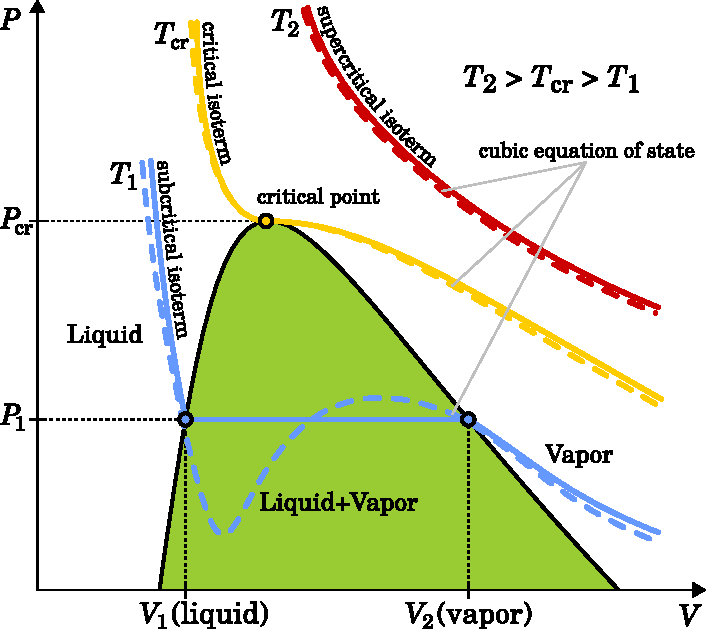
\includegraphics[width=10cm]{figures/phase-diagram-pv-cubic-eos}
\par\end{centering}
\caption{\label{fig:phase-diagram-pv}A pressure-volume phase diagram for a
substance. Dashed lines correspond to a cubic equation of state modeling
the $PVT$ behavior of the substance.}
\end{figure}

To correct for the non-ideal thermodynamic behavior of gases, more
accurate equations of state need to be used. These equations govern
the mutual dependency on temperature, $T$, pressure, $P$, and molar
volume, $V$, with the equation of state for an ideal gas being the
simplest one:
\[
\frac{PV}{RT}=1.
\]
In this project, the following \emph{general cubic equation of state}
needs to be used \citep[see][p. 93, eq. 3.42]{Smith2005}:
\begin{equation}
P=\frac{RT}{V-b}-\frac{a(T,\omega)}{(V+\epsilon b)(V+\sigma b)},\label{eq:cubic-eos}
\end{equation}
where $\epsilon$ and $\sigma$ are given constants (see their values
for different equation of state models in Table~\ref{tab:eos-params}),
and $a$ and $b$ are:
\begin{align}
a(T) & \coloneqq\Psi\frac{\alpha(T_{\mathrm{r}},\omega)R^{2}T_{\mathrm{c}}^{2}}{P_{\mathrm{c}}},\\
\shortintertext{and}b & \coloneqq\Omega\frac{RT_{\mathrm{c}}}{P_{\mathrm{c}}},
\end{align}
with $T_{\mathrm{c}}$ and $P_{\mathrm{c}}$ denoting the \emph{critical
temperature} and \emph{critical pressure} of the gas; $\Psi$ and
$\Omega$ given constants and $\alpha(T_{\mathrm{r}},\omega)$ a given
function, each of these varying with the equation of state model (see
Table~\ref{tab:eos-params}); $T_{\mathrm{r}}$ and $P_{\mathrm{r}}$
denoting the \emph{reduced temperature} and \emph{reduced pressure},
respectively, of the substance:
\begin{equation}
T_{\mathrm{r}}=\frac{T}{T_{\mathrm{c}}}\qquad\text{and}\qquad P_{\mathrm{r}}=\frac{P}{P_{\mathrm{c}}},
\end{equation}
and $\omega$ the \emph{acentric factor} of the substance, needed
in the evaluation of function $\alpha(T_{\mathrm{r}},\omega)$ for
some models (see Table~\ref{tab:eos-params}), with ${\omega=0.224}$
for CO$_{2}$. 

\begin{algorithm}[t]
\caption{\label{alg:comp-factor-gas-fixed-point}Fixed-point algorithm for
the compressibility factor calculation.}

\setstretch{1.5}
\begin{algorithmic}[1]

\Function{CompressibilyFactor}{$T, P; T_\mathrm{c}, P_\mathrm{c}, \Psi, \Omega, \omega$}
  \State $T_\mathrm{r} \gets T/T_\mathrm{c}$
  \State $P_\mathrm{r} \gets P/P_\mathrm{c}$
  \State $\alpha \gets \alpha(T_\mathrm{r},\omega)$ \Comment{See Table~\ref{tab:eos-params} for function $\alpha(T_\mathrm{r},\omega)$ for different models.}  
  \State $\beta \gets \Omega\frac{P_{\mathrm{r}}}{T_{\mathrm{r}}}$ \Comment{Using Eq.~(\ref{eq:cubic-eos-beta}).}
  \State $q \gets \frac{\Psi}{\Omega}\frac{\alpha}{T_{\mathrm{r}}}$ \Comment{Using Eq.~(\ref{eq:cubic-eos-q}).}
  \State $Z \gets 1$ \Comment{Initial guess for $Z$ corresponding to the compressibility factor of an ideal gas.}
  \For{$i \gets 1 \textrm{ to } i_\textrm{max}$}
     \State $Z_\textrm{new} \gets 1+\beta-q\beta\frac{Z-\beta}{(Z+\epsilon\beta)(Z+\sigma\beta)}$ \Comment{Using Eq.~(\ref{eq:cubic-eos-reduced-vapor-root}).}
	 \If{$|Z_\textrm{new}-Z|/Z < \epsilon_\textrm{tol}$} \Comment{We stop when $Z_\textrm{new}$ is relatively close enough to $Z$.}
       \State \Return{$Z_\textrm{new}$}
	 \EndIf
     \State $Z \gets Z_\textrm{new}$
  \EndFor
  \State \textbf{throw} \emph{Error: Calculation failed to converge.}
\EndFunction

\end{algorithmic}
\end{algorithm}

\begin{algorithm}[t]
\caption{\label{alg:comp-factor-gas-newton}Newton's method for the compressibility
factor calculation.}

\setstretch{1.5}
\begin{algorithmic}[1]

\Function{CompressibilyFactor}{$T, P; T_\mathrm{c}, P_\mathrm{c}, \Psi, \Omega, \omega$}
  \State $T_\mathrm{r} \gets T/T_\mathrm{c}$
  \State $P_\mathrm{r} \gets P/P_\mathrm{c}$
  \State $\alpha \gets \alpha(T_\mathrm{r},\omega)$ \Comment{See Table~\ref{tab:eos-params} for function $\alpha(T_\mathrm{r},\omega)$ for different models.}  
  \State $\beta \gets \Omega\frac{P_{\mathrm{r}}}{T_{\mathrm{r}}}$ \Comment{Using Eq.~(\ref{eq:cubic-eos-beta}).}
  \State $q \gets \frac{\Psi}{\Omega}\frac{\alpha}{T_{\mathrm{r}}}$ \Comment{Using Eq.~(\ref{eq:cubic-eos-q}).}
  \State $Z \gets 1$ \Comment{Initial guess for $Z$ corresponding to the compressibility factor of an ideal gas.}
  \For{$i \gets 1 \textrm{ to } i_\textrm{max}$}
     \State $f_Z \gets 1+\beta-q\beta\frac{Z-\beta}{(Z+\epsilon\beta)(Z+\sigma\beta)}-Z$
     \State $f^{\prime}_{Z} \gets -\frac{q\beta}{(Z+\epsilon\beta)(Z+\sigma\beta)}\left\{ 1-(Z-\beta)\frac{2Z+(\epsilon+\sigma)\beta}{(Z+\epsilon\beta)(Z+\sigma\beta)}\right\} -1$
     \State $Z_\textrm{new} \gets Z - f_Z/f^{\prime}_{Z}$ 
	 \If{$f_Z < \epsilon_\textrm{tol}$} \Comment{We stop when $f(Z)$ is sufficiently close to zero.}
       \State \Return{$Z_\textrm{new}$}
	 \EndIf
     \State $Z \gets Z_\textrm{new}$
  \EndFor
  \State \textbf{throw} \emph{Error: Calculation failed to converge.}
\EndFunction

\end{algorithmic}
\end{algorithm}

Every substance has a different critical temperature, $T_{\mathrm{c}}$,
and critical pressure, $P_{\mathrm{c}}$. When the temperature and
pressure of the substance is greater than their respective critical
values, the substance is then said to be in a \emph{supercritical
state}. This is a physical state in which the substance behaves similarly
to a liquid and gas (e.g., the substance is dense, like a liquid,
and has low viscosity, like a gas). The critical temperature and pressure
of CO$_{2}$ are 304.2~K and 73.83~bar, respectively.

Equation (\ref{eq:cubic-eos}) can be more conveniently written in
terms of the \emph{compressibility factor}, $Z$, of the gaseous solution,
with $Z$ defined as: 
\begin{equation}
Z\coloneqq\frac{PV}{RT}.
\end{equation}
After some algebraic manipulations, the following equation can be
derived in terms of $Z$ only:
\begin{equation}
Z=\frac{Z}{Z-\beta}-q\beta\frac{Z}{(Z+\epsilon\beta)(Z+\sigma\beta)},\label{eq:cubic-eos-reduced}
\end{equation}
where $\beta$ and $q$ are defined as:
\begin{align}
\beta & \coloneqq\Omega\frac{P_{\mathrm{r}}}{T_{\mathrm{r}}}\label{eq:cubic-eos-beta}\\
\shortintertext{and}q & \coloneqq\frac{\Psi}{\Omega}\frac{\alpha(T_{\mathrm{r}},\omega)}{T_{\mathrm{r}}}.\label{eq:cubic-eos-q}
\end{align}

We will use Eq.~(\ref{eq:cubic-eos-reduced}) to calculate $Z$ for
a given temperature $T$ and pressure $P$. Since Eq.~(\ref{eq:cubic-eos-reduced})
is a cubic polynomial:
\[
Z^{3}+AZ^{2}+BZ+C=0,
\]
(\textbf{Exercise:} Determine the coefficient $A$, $B$, $C$ in
terms of $\beta$ and $q$.) it follows that there exists three values
for $Z$ that satisfies that equation (i.e., three roots). When these
three roots are real numbers (there could be only one real root and
a conjugate pair of complex roots!), the smallest value corresponds
to a liquid state, and the largest value corresponds to a gas state.
The middle value is not physically relevant (see Figure~\ref{fig:phase-diagram-pv}).
Since we are interested in calculating the fugacity coefficient of
CO$_{2}$(g) in this project, we should then require only the largest
root of Eq.~(\ref{eq:cubic-eos-reduced}). For this, it is numerically
convenient to write Eq.~(\ref{eq:cubic-eos-reduced}) in the following
form \citep[see][p. 97, eq. 3.52]{Smith2005}:
\begin{equation}
Z=1+\beta-q\beta\frac{Z-\beta}{(Z+\epsilon\beta)(Z+\sigma\beta)}.\label{eq:cubic-eos-reduced-vapor-root}
\end{equation}
A simple \emph{fixed-point iterative algorithm} to find $Z$ that
solves Eq.~(\ref{eq:cubic-eos-reduced-vapor-root}) is given in Algorithm~\ref{alg:comp-factor-gas-fixed-point}.
This method, however, is not very efficient and robust. Thus, \emph{Newton's
method} is preferred.

In Newton's method, we transform the non-linear equation in Eq.~(\ref{eq:cubic-eos-reduced-vapor-root})
into the form: 
\begin{equation}
f(Z)=0,
\end{equation}
where $f$ is the \emph{residual function} defined as:
\begin{equation}
f(Z)=1+\beta-q\beta\frac{Z-\beta}{(Z+\epsilon\beta)(Z+\sigma\beta)}-Z.
\end{equation}
Newton's method requires $f^{\prime}(Z)$, the first order derivative
of $f$:
\begin{equation}
f^{\prime}(Z)=-\frac{q\beta}{(Z+\epsilon\beta)(Z+\sigma\beta)}\left\{ 1-(Z-\beta)\frac{2Z+(\epsilon+\sigma)\beta}{(Z+\epsilon\beta)(Z+\sigma\beta)}\right\} -1.
\end{equation}

The iterative procedure in Newton's method is as follows: start with
an initial guess for $Z$, say $Z^{0}=1$. Then, perform the following
iterative steps:
\begin{align}
Z^{1} & =Z^{0}-f(Z^{0})/f^{\prime}(Z^{0}) & \qquad & 1^{\text{st}}\text{ iteration}\nonumber \\
 & \hphantom{=1+\beta-q\beta}\vdots &  & \qquad\vdots\\
Z^{i+1} & =Z^{i}-f(Z^{i})/f^{\prime}(Z^{i}) &  & i^{\text{th}}\text{ iteration}\nonumber 
\end{align}
until iteration $i$ that satisfies:
\begin{equation}
f(Z^{i+1})<\epsilon_{\mathrm{tol}},
\end{equation}
where $\epsilon_{\mathrm{tol}}$ is a tolerance, say, $\epsilon_{\mathrm{tol}}=10^{-4}$,
for the residual function $f$. See Algorithm~\ref{alg:comp-factor-gas-newton}
for a more detailed description of the required steps to calculate
$Z$ using Newton's method.

Once $Z$ is calculated, we can calculate the fugacity coefficient
of the gas using:
\begin{equation}
\boxed{\ln\varphi_{i}\coloneqq Z-1-\ln(Z-\beta)-q\theta},
\end{equation}
where $\theta$ is defined as:
\begin{equation}
\theta\coloneqq\begin{cases}
{\displaystyle \frac{1}{\sigma-\epsilon}\ln\left(\frac{Z+\sigma\beta}{Z+\epsilon\beta}\right)} & \epsilon\neq\sigma\\
{\displaystyle \frac{\beta}{Z+\epsilon\beta}}^{^{^{^{^ {}}}}} & \epsilon=\sigma
\end{cases}.
\end{equation}


\section{Implementing interpolation function for standard chemical potentials\label{subsec:Implementing-interpolation-funct}}

\begin{table}
\caption{\label{tab:standard-chemical-potentials}The standard chemical potentials
of the chemical species, $\mu_{i}^{\circ}$, considered in this project,
in J/mol. These values were calculated by Reaktoro \citep{Leal2015b}
using the SUPCRT92 \citep{Johnson1992} database \texttt{slop98.dat}.}
\footnotesize

\begin{tabular*}{1\columnwidth}{@{\extracolsep{\fill}}ccccc}
\toprule 
\multirow{2}{*}{} & \multirow{2}{*}{$T$ {[}°C{]}} & \multicolumn{3}{c}{$P$ {[}bar{]}}\tabularnewline
\cmidrule{3-5} \cmidrule{4-5} \cmidrule{5-5} 
 &  & 1 & 50 & 100\tabularnewline
\midrule
\multirow{4}{*}{H$_{2}$O(l)} & 25 & -237181.72 & -237093.28 & -237003.23\tabularnewline
 & 50 & -239006.71 & -238917.46 & -238826.59\tabularnewline
 & 75 & -240977.57 & -240887.12 & -240795.03\tabularnewline
 & 100 & \textemdash{} & -242992.18 & -242898.53\tabularnewline
\midrule 
\multirow{4}{*}{H$^{+}$(aq)} & 25 & 0 & 0 & 0\tabularnewline
 & 50 & 0 & 0 & 0\tabularnewline
 & 75 & 0 & 0 & 0\tabularnewline
 & 100 & \textemdash{} & 0 & 0\tabularnewline
\midrule 
\multirow{4}{*}{OH$^{-}$(aq)} & 25 & -157297.48 & -157320.08 & -157342.16\tabularnewline
 & 50 & -156905.20 & -156924.41 & -156943.13\tabularnewline
 & 75 & -156307.81 & -156328.46 & -156348.60\tabularnewline
 & 100 & \textemdash{} & -155558.52 & -155583.77\tabularnewline
\midrule 
\multirow{4}{*}{HCO$_{3}^{-}$(aq)} & 25 & -586939.89 & -586820.91 & -586698.78\tabularnewline
 & 50 & -589371.68 & -589247.85 & -589120.88\tabularnewline
 & 75 & -591758.94 & -591634.79 & -591507.48\tabularnewline
 & 100 & \textemdash{} & -593983.38 & -593858.95\tabularnewline
\midrule 
\multirow{4}{*}{CO$_{3}^{2-}$(aq)} & 25 & -527983.14 & -528011.90 & -528039.31\tabularnewline
 & 50 & -526461.60 & -526494.20 & -526525.56\tabularnewline
 & 75 & -524473.15 & -524514.70 & -524555.01\tabularnewline
 & 100 & \textemdash{} & -522121.51 & -522175.91\tabularnewline
\midrule 
\multirow{4}{*}{CO$_{2}$(aq)} & 25 & -385974.00 & -385813.47 & -385650.13\tabularnewline
 & 50 & -389147.04 & -388979.61 & -388809.39\tabularnewline
 & 75 & -392728.17 & -392556.66 & -392382.38\tabularnewline
 & 100 & \textemdash{} & -396484.88 & -396307.90\tabularnewline
\midrule 
\multirow{4}{*}{Na$^{+}$(aq)} & 25 & -261880.74 & -261886.18 & -261890.73\tabularnewline
 & 50 & -263384.24 & -263384.84 & -263384.60\tabularnewline
 & 75 & -264979.92 & -264978.35 & -264975.97\tabularnewline
 & 100 & \textemdash{} & -266664.71 & -266661.71\tabularnewline
\midrule 
\multirow{4}{*}{Cl$^{-}$(aq)} & 25 & -131289.74 & -131204.66 & -131117.63\tabularnewline
 & 50 & -132590.59 & -132504.28 & -132416.09\tabularnewline
 & 75 & -133682.46 & -133598.32 & -133512.30\tabularnewline
 & 100 & \textemdash{} & -134501.87 & -134420.82\tabularnewline
\midrule 
\multirow{4}{*}{Ca$^{2+}$(aq)} & 25 & -552790.08 & -552879.51 & -552968.88r\tabularnewline
 & 50 & -551348.98 & -551437.62 & -551526.28\tabularnewline
 & 75 & -549855.33 & -549945.95 & -550036.62\tabularnewline
 & 100 & \textemdash{} & -548400.71 & -548495.68\tabularnewline
\midrule 
\multirow{4}{*}{CO$_{2}$(g)} & 25 & -394358.74 & -394358.74 & -394358.74\tabularnewline
 & 50 & -399740.71 & -399740.71 & -399740.71\tabularnewline
 & 75 & -405197.73 & -405197.73 & -405197.73\tabularnewline
 & 100 & -410726.87 & -410726.87 & -410726.87\tabularnewline
\midrule 
\multirow{4}{*}{CaCO$_{3}$(s,calcite)} & 25 & -1129177.92 & -1128996.94 & -1128812.26\tabularnewline
 & 50 & -1131580.05 & -1131399.06 & -1131214.39\tabularnewline
 & 75 & -1134149.89 & -1133968.91 & -1133784.23\tabularnewline
 & 100 & -1136882.60 & -1136701.62 & -1136516.94\tabularnewline
\bottomrule
\end{tabular*}

\smallskip{}

\footnotesize

\textbf{Note:} At 100~°C and 1~bar, water is in vapor state, and
thus a dash ``\textemdash '' is used for the values of $\mu_{i}^{\circ}$
for aqueous species at that temperature and pressure condition. What
could be an appropriate value to use in the Python code for those
entries?
\end{table}

The provided Python code is limited to calculate the solubility of
CO$_{2}$ and CaCO$_{3}$ at 25~°C and 1~bar only. This is because
the code only uses \emph{standard chemical potentials of the species},
$\mu_{i}^{\circ}$, at that temperature and pressure values. 

Table~\ref{tab:standard-chemical-potentials} contains the standard
chemical potentials of all species in Table~\ref{tab:chemical-system-example}
at temperatures 25, 50, 75, and 100~°C and pressures 1, 50, 100~bar.
In this project, $\mu_{i}^{\circ}$ at a given $T$ and $P$ needs
to be interpolated from the given values of $\mu_{i}^{\circ}$ at
those temperature and pressure points. In what follows, we describe
how this interpolation calculation can be performed in general.

Let $f(x,y)$ be a function defined over the region $[x_{L},x_{R}]\times[y_{B},y_{T}]$
and let $f_{ij}$ denote its tabulated value at the discrete coordinate
point $(x_{i},y_{j})$ (see Figure~\ref{fig:lagrange-interpolation}).
Here, $x_{i}$ denotes the $x$-coordinate of the $i$th point in
the discretization of the range $[x_{L},x_{R}]$, and $y_{j}$ the
$y$-coordinate of the $j$th point in the the discretization of the
range $[y_{B},y_{T}]$. If $(x,y)$ is the point where the value of
$f$ needs to be interpolated, i.e., where $f(x,y)$ is needed, with
$x\in[x_{L},x_{R}]$ and $y\in[y_{B},y_{T}]$, then one can use the
following first order Lagrange interpolation formula:
\begin{equation}
f(x,y)=f_{i,j}+\frac{x-x_{i}}{x_{i+1}-x_{i}}(f_{i+1,j}-f_{i,j})+\frac{y-y_{j}}{y_{j+1}-y_{j}}(f_{i,j+1}-f_{i,j}).\label{eq:lagrange-interpolation-1st-order}
\end{equation}

The above formula can be used to calculate $\mu_{i}^{\circ}(T,P)$
using tabulated values of $\mu_{i}^{\circ}$ over a set of given temperature
and pressure points. The coordinates $x$ and $y$ above correspond
to temperature and pressure, and the function $f$ corresponds to
standard chemical potentials of the species, $\mu_{i}^{\circ}$.

\begin{figure}
\centering{}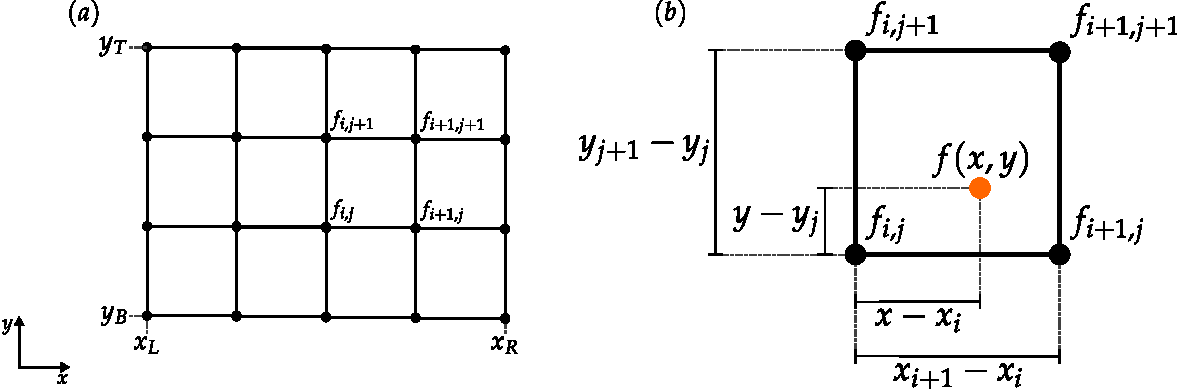
\includegraphics[width=1\textwidth]{figures/lagrange-interpolation}
\caption{\label{fig:lagrange-interpolation}Illustration of the tabulated values
of function $f$ and how it. \emph{(a)}~The grid where the values
of function $f$ are tabulated over the black bullet points. \emph{(b)~}The
use of the first order Lagrange interpolation scheme to interpolate
$f$ at the red point at $(x,y)$.}
\end{figure}


\section{Explanation about the Python code}

\begin{figure}
\begin{centering}
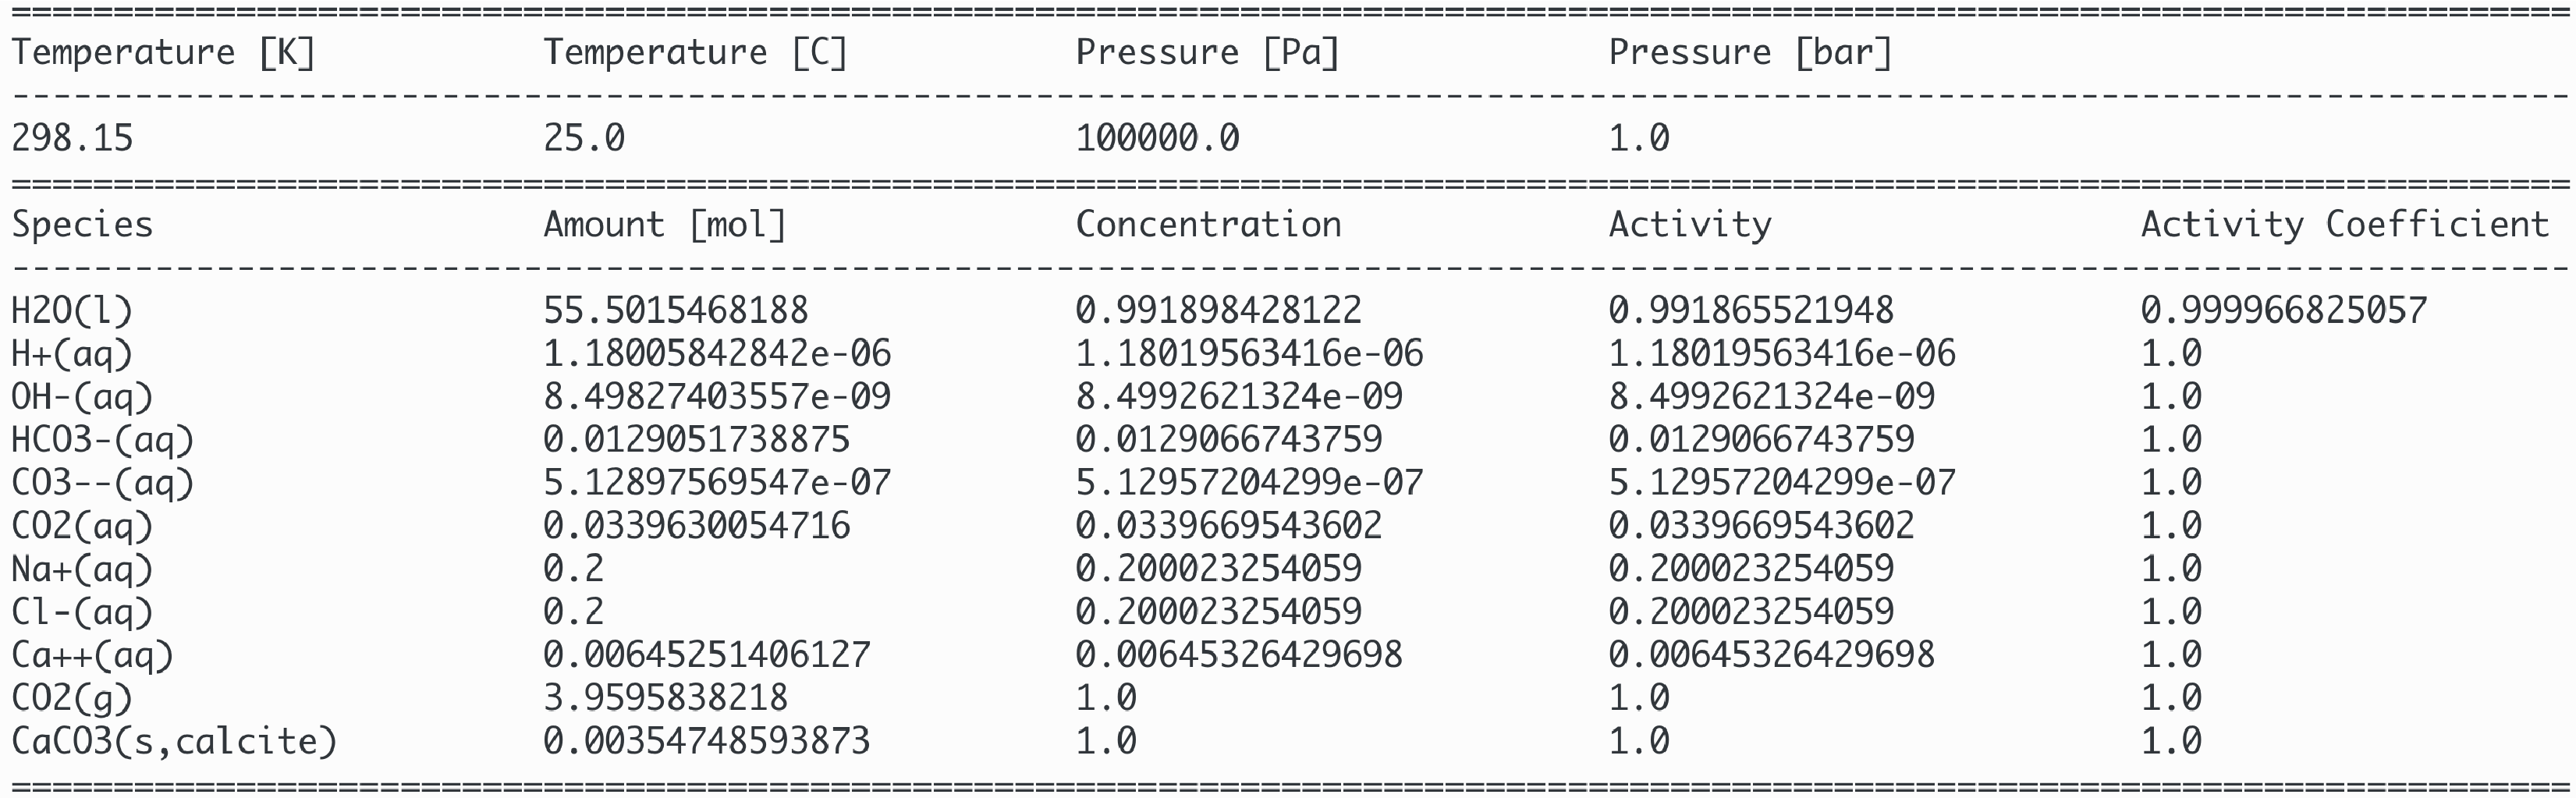
\includegraphics[width=1\textwidth]{figures/project-output-results-demo}
\par\end{centering}
\caption{\label{fig:output-results}The file \texttt{results.txt} that is output
by executing the Python code \texttt{project.py}.}
\end{figure}

The provided Python code, \texttt{project.py}, can be executed in
your machine or in some website that provides a development environment
for Python, such as \texttt{repl.it} at:

\begin{minipage}[t]{1\columnwidth}%
\begin{center}
\texttt{\href{https://repl.it/languages/python}{https://repl.it/languages/python}}
\par\end{center}%
\end{minipage}

If you prefer to run it locally, in your machine, you will need to
install Python 2.7, if it isn't already natively provided by your
operating system, like it is in Linux and MacOS. For Windows users,
you can find the Python installer at: \texttt{}~\\
\texttt{}%
\begin{minipage}[t]{1\columnwidth}%
\begin{center}
\texttt{\href{https://www.python.org/downloads/release/python-2713/}{https://www.python.org/downloads/release/python-2713/}}
\par\end{center}%
\end{minipage}

Once Python is available in your machine, you can execute the file
\texttt{project.py} in a terminal:\texttt{}~\\
\texttt{}%
\begin{minipage}[t]{1\columnwidth}%
\begin{center}
\texttt{python project.py}
\par\end{center}%
\end{minipage}\\
with the assumption that the current directory in the terminal is
where the file \texttt{project.py} is located. If not, use the command
\texttt{cd} to change to the right directory. Alternatively, you can
install the SublimeText editor, open \texttt{project.py}, and press
$\mathrm{Ctrl+b}$. 

In both cases, a file \texttt{results.txt} should be output in the
same directory. The contents of this file should be similar to what
is shown in Figure~\ref{fig:output-results}. The output file show
the temperature and pressure inputs, and the resulting equilibrium
state, listing the molar amounts, concentrations, activities, and
activity coefficients of the species. Note that in the output file
that activity coefficients, $\gamma_{i}$, of the aqueous species
and the fugacity coefficient, $\varphi_{i}$, of CO$_{2}$(g) is one
(last column of the table in Figure~\ref{fig:output-results}), so
that the calculated equilibrium state should not be accurate since
the thermodynamic behavior of the aqueous solution and CO$_{2}$(g)
is modeled using ideal models.

At the bottom of \texttt{project.py} file, you should see a function
with the following signature and return statement:

\begin{lstlisting}[language=Python, caption=Function of chemical equilibrium algorithm]
def equilibrate(T, P, b):
    ...
    return equilibriumstate
\end{lstlisting}
%\begin{figure}[H]
%\begin{pythoncode}
%def equilibrate(T, P, b):
%    ...
%    return equilibriumstate
%\end{pythoncode}
%\end{figure}

In this function, \texttt{T} is temperature in K, \texttt{P} is pressure
in Pa, and \texttt{b} is an array with the molar amounts of the elements.
The returned object, \texttt{equilibriumstate}, contains (or stores)
the temperature and pressure used in the calculation, the amounts,
concentrations, activities, and activity coefficients of the species.
The following is the usage to perform an equilibrium calculation and
the subsequent calls t:

\begin{lstlisting}[language=Python, caption=Perform an equilibrium calculation]
	# Perform an equilibrium calculation with given T, P, b 
	# and store the result in object `state`. 
	# Here `state` is just a name to the object containing 
	# the calculated equilibrium state data. 
	# One could have chosen a different name, like `mystate`.
	state = equilibrate(T, P, b)
	
	# To extract data from object `state`, use the following statements:
	state.T  # access the temperature stored in the returned `state` object
	state.P  # access the pressure stored in the returned `state` object
	state.n  # access the molar amounts (array) of the species in `state`
	state.c  # access the concentrations (array) of the species in `state`
	state.a  # access the activities (array) of the species in `state`
	state.g  # access the activity coefficients (array) in `state`
\end{lstlisting}

%\begin{figure}[H]
%\begin{pythoncode}
%# Perform an equilibrium calculation with given T, P, b 
%# and store the result in object `state`. 
%# Here `state` is just a name to the object containing 
%# the calculated equilibrium state data. 
%# One could have chosen a different name, like `mystate`.
%state = equilibrate(T, P, b)
%
%# To extract data from object `state`, use the following statements:
%state.T  # access the temperature stored in the returned `state` object
%state.P  # access the pressure stored in the returned `state` object
%state.n  # access the molar amounts (array) of the species in `state`
%state.c  # access the concentrations (array) of the species in `state`
%state.a  # access the activities (array) of the species in `state`
%state.g  # access the activity coefficients (array) in `state`
%\end{pythoncode}
%\end{figure}

Because we want to perform equilibrium calculations using inputs of
the form: 1~kg of H$_{2}$O, 1~mol of CO$_{2}$, 0.5~moles of NaCl,
5~moles of CaCO$_{3}$, \texttt{project.py} provides the utility
function:

\begin{lstlisting}[language=Python, caption=$component_amounts()$ function]
	def component_amounts(kgH2O, molCO2, molNaCl, molCaCO3):
	...
	return b
\end{lstlisting}

%\begin{figure}[H]
%\begin{pythoncode}
%def component_amounts(kgH2O, molCO2, molNaCl, molCaCO3):
%    ...
%    return b
%\end{pythoncode}
%\end{figure}

which can be used as follows in an example to calculate the pH of
the aqueous solution:

%\begin{figure}[H]
%\begin{pythoncode}
%T = 333.15  # temperature in K (=60 C)
%P = 100e5  # pressure in Pa (=100 bar)
%# Calculate the amounts of elements based on a mixture of 
%# 1 kg of H2O, 1 mol of CO2, 0.5 moles of NaCl, and 5 moles of CaCO3.
%b = component_amounts(kgH2O=1, molCO2=1, molNaCl=0.5, molCaCO3=5)
%state = equilibrate(T, P, b)  # perform the equilibrium calculation
%iH = species.index('H+(aq)')  # the index of species H+(aq)
%pH = -log10(state.a[iH])  # calculate the pH of the aqueous solution
%print 'The pH in the calculated equilibrium state is', pH
%\end{pythoncode}
%\end{figure}

\begin{lstlisting}[language=Python, caption=Calculate pH]
	T = 333.15  # temperature in K (=60 C)
	P = 100e5  # pressure in Pa (=100 bar)
	# Calculate the amounts of elements based on a mixture of 
	# 1 kg of H2O, 1 mol of CO2, 0.5 moles of NaCl, and 5 moles of CaCO3.
	b = component_amounts(kgH2O=1, molCO2=1, molNaCl=0.5, molCaCO3=5)
	state = equilibrate(T, P, b)  # perform the equilibrium calculation
	iH = species.index('H+(aq)')  # the index of species H+(aq)
	pH = -log10(state.a[iH])  # calculate the pH of the aqueous solution
	print 'The pH in the calculated equilibrium state is', pH
\end{lstlisting}

One of the figures to be plot as part of this project is a pH versus
amount of CO$_{2}$ (see Figure~\ref{fig:assigned-figures}). In
this figure, a series of equilibrium calculations need to be performed
at 75~°C and 100~bar. In this series of calculations, the idea is
to mix an increasing amount of CO$_{2}$, from 0 to 2 moles, with
1~kg of H$_{2}$O and 0.3~mol of NaCl (which should produce an aqueous
solution with 0.3 NaCl molal as required). You should decide how many
increasing steps for the amount of CO$_{2}$. At each calculation,
the pH of the solution should then be calculated by accessing the
calculated equilibrium state data; collecting the activity of species
H$^{+}$(aq), $a_{\mathrm{H^{+}(aq)}}$; and then calculating ${\mathrm{pH}=-\log_{10}(a_{\mathrm{H^{+}(aq)}})}$.
For this plot, the $x$-axis is the amount of CO$_{2}$, varying from
0 to 2 moles, and the $y$-axis is the calculated pH. 

For all other figures, a similar procedure should be performed: perform
a series of equilibrium calculations by adequately varying the inputs
(e.g., temperature, pressure, amounts of CO$_{2}$, NaCl, CaCO$_{3}$,
etc.) and then extract from the calculated equilibrium state the proper
quantities that will serve for its immediate use in a plot, or used
to calculate another quantity of interest (e.g., pH).

\section{Grading}

The maximum grade of this project is \textbf{100 points}. If the required
corrections in the Python code are not properly implemented, the maximum
grade you will be able to get is \textbf{80 points}. The following
shows how many points each correction contributes to the maximum grade
you can have:
\begin{itemize}
\item \textbf{5~points} if the Peng\textendash Robinson model is incorporated
for the activity of CO$_{2}$(g);
\item \textbf{5~points} if the Davies model is incorporated for the activity
coefficients of ionic species;
\item \textbf{5~points} if the Drummond model is incorporated for the activity
coefficient of species CO$_{2}$(aq);
\item \textbf{5~points} if the figures are produced with standard chemical
potentials corrected for temperatures and pressures other than 25~°C
and 1~bar.
\end{itemize}
Thus, by resolving all the above issues, you can achieve the maximum
100 points. The explanation of the figures in the written report is
important in your final grade.

\section{Assistance}

Should you need help with Python coding and\slash or further explanation
of the thermodynamic concepts involved in this project, do not hesitate
to contact me. 

\bibliographystyle{apalike}
\bibliography{../library}

\end{document}
